\definecolor{class1}{RGB}{228,26,28}
\definecolor{class2}{RGB}{55,126,184}
\definecolor{class3}{RGB}{77,175,74}
\definecolor{class4}{RGB}{152,78,163}
\definecolor{class5}{RGB}{255,127,0}

\tikzset{wagon/.style={draw = gray, ultra thick, opacity = 0.7}}
\tikzset{class1/.style={draw = class1, ultra thick, opacity = 1}}
\tikzset{class2/.style={draw = class2, ultra thick, opacity = 1}}
\tikzset{class3/.style={draw = class3, ultra thick, opacity = 1}}
\tikzset{class4/.style={draw = class4, ultra thick, opacity = 1}}
\tikzset{class5/.style={draw = class5, ultra thick, opacity = 1}}
\tikzset{annotation/.style={draw = black, thick, opacity = 0.7}}


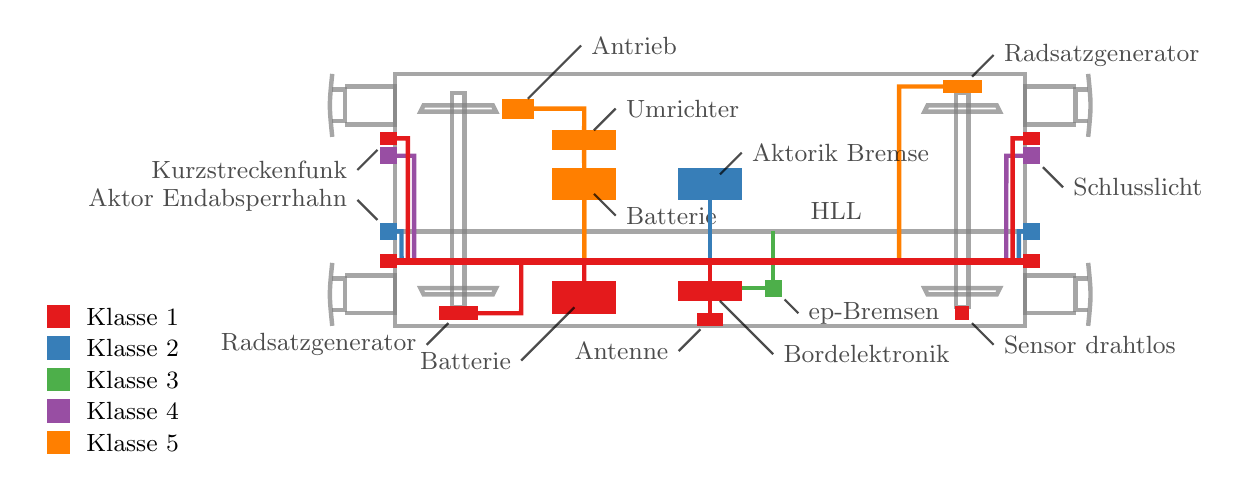
\begin{tikzpicture}[font = \sffamily, scale = 0.8]
\tikzstyle{every node}=[font=\small]
\path[class5, fill = none, draw = none] (-3.3, 1.3) rectangle +(.5,.3) node[pos = 0.5] (dri) {};
\path[annotation, draw = none, opacity = 0] (dri) -- +(1,1) node[right] {Antrieb};
    {%wagon as basis
    \path[wagon] (-5,-2) -- (-5,2) -- (5,2) -- (5,-2) -- cycle;
    % HL
    \path[wagon] (-5,-.5) -- (5,-.5) node[pos = 0.7, above] {HLL};
    % Buffer
    \begin{scope}[shift = {(-5,1.5)}]
    	\path[wagon] (-.8,.3) -- (0,.3) -- (0,-.3) -- (-.8,-.3);
    	\path[wagon] (-1,.25) -- (-.8,.25) -- (-.8,-.25) -- (-1,-.25);
    	\path[wagon] (-1,-.5) .. controls (-1.05,0) and (-1.05,0) .. (-1,.5);
    \end{scope}
    \begin{scope}[shift = {(-5,-1.5)}]
    	\path[wagon] (-.8,.3) -- (0,.3) -- (0,-.3) -- (-.8,-.3);
    	\path[wagon] (-1,.25) -- (-.8,.25) -- (-.8,-.25) -- (-1,-.25);
    	\path[wagon] (-1,-.5) .. controls (-1.05,0) and (-1.05,0) .. (-1,.5);
    \end{scope}
    \begin{scope}[shift = {(5,-1.5)}, rotate = 180]
    	\path[wagon] (-.8,.3) -- (0,.3) -- (0,-.3) -- (-.8,-.3);
    	\path[wagon] (-1,.25) -- (-.8,.25) -- (-.8,-.25) -- (-1,-.25);
    	\path[wagon] (-1,-.5) .. controls (-1.05,0) and (-1.05,0) .. (-1,.5);
    \end{scope}
    \begin{scope}[shift = {(5,1.5)}, rotate = 180]
    	\path[wagon] (-.8,.3) -- (0,.3) -- (0,-.3) -- (-.8,-.3);
    	\path[wagon] (-1,.25) -- (-.8,.25) -- (-.8,-.25) -- (-1,-.25);
    	\path[wagon] (-1,-.5) .. controls (-1.05,0) and (-1.05,0) .. (-1,.5);
    \end{scope}
    %Wheelset
    \begin{scope}[shift = {(-4,0)}]
    	\path[wagon] (-.1,1.7) -- (.1,1.7) -- (.1,-1.7) -- (-.1, -1.7) -- cycle; 
    	\path[wagon] (-.6,1.4) -- (.6,1.4) -- (.55,1.5) -- (-.55, 1.5) -- cycle; 
    	\path[wagon] (-.6,-1.4) -- (.6,-1.4) -- (.55,-1.5) -- (-.55, -1.5) -- cycle; 
    \end{scope}
    \begin{scope}[shift = {(4,0)}]
    	\path[wagon] (-.1,1.7) -- (.1,1.7) -- (.1,-1.7) -- (-.1, -1.7) -- cycle; 
    	\path[wagon] (-.6,1.4) -- (.6,1.4) -- (.55,1.5) -- (-.55, 1.5) -- cycle; 
    	\path[wagon] (-.6,-1.4) -- (.6,-1.4) -- (.55,-1.5) -- (-.55, -1.5) -- cycle; 
    \end{scope}}
    
    % Class 5
    {
    %Wheelset generator
    \path[class5, fill = class5, thin] (4.3, 1.9) rectangle +(-.6,-.2) node[pos = 0.5] (wsg2) {};
    \path[class5] (wsg2) +(-.1,0) -- +(-1,0) -- (3,-1);
    \path[annotation] (wsg2) -- +(.5,.5) node[right] {Radsatzgenerator};
    %Battery
    \path[class5, fill = class5, thin] (-2.5, 0) rectangle +(1,.5) node[pos = 0.5] (bat2) {};
    \path[class5] (bat2) +(0,0)  -- (-2,-1);
    \path[annotation] (bat2) -- +(.5,-.5) node[right] {Batterie};
    %Converter
    \path[class5, fill = class5, thin] (-2.5, .8) rectangle +(1,.3) node[pos = 0.5] (con) {};
    \path[class5] (con) +(0,0)  -- (-2,-1);
    \path[annotation] (con) -- +(.5,.5) node[right] {Umrichter};
    %Drive
    \path[class5, fill = class5, thin] (-3.3, 1.3) rectangle +(.5,.3) node[pos = 0.5] (dri) {};
    \path[class5] (dri)  -- (-2,1.45) -- (con);
    \path[annotation] (dri) -- +(1,1) node[right] {Antrieb};
    }
    % Class 4
    {
    \path[class4, fill = class4] (-5.2, .6) rectangle (-5,.8) node[pos = 0.5] (eota) {};
    \path[class4, fill = class4] (5.2, .6) rectangle (5,.8) node[pos = 0.5] (eotb) {};
    \path[class4] (eota) +(-.1,0) -- +(.4,0) -- (-4.7,-1);
    \path[class4] (eotb) +(.1,0) -- +(-.4,0) -- (4.7,-1);
    \path[annotation] (eotb) -- +(.5,-.5) node[right] {Schlusslicht};
    }
    % Class 3
    {
    \path[class3] (1,-.5) -- (1,-1.3);
    \path[class3, fill = class3] (.9,-1.3) rectangle (1.1,-1.5) node[pos = 0.5] (epb) {};
    \path[class3] (epb) +(.1,0) -- +(-.5,0);
    \path[annotation] (epb) -- +(.4,-.4) node[right] {ep-Bremsen};
    }
    %Class 2
    {%End cocks
    \path[class2, fill = class2] (-5.2, -.4) rectangle (-5,-.6) node[pos = 0.5] (eca) {};
    \path[class2, fill = class2] (5.2, -.4) rectangle (5,-.6) node[pos = 0.5] (ecb) {};
    \path[class2] (eca) +(-.1,0) -- +(.2,0) -- (-4.9,-1);
    \path[class2] (ecb) +(.1,0) -- +(-.2,0) -- (4.9,-1);
    \path[annotation] (eca) -- +(-.5,.5) node[left] {Aktor Endabsperrhahn};
    %Battery
    \path[class2, fill = class2, thin] (-.5, 0) rectangle +(1,.5) node[pos = 0.5] (bcu) {};
    \path[class2] (bcu) +(0,0)  -- (0,-1);
    \path[annotation] (bcu) -- +(.5,.5) node[right] {Aktorik Bremse};
    }
    
    {%class 1
    %Tube
    \path[class1] (-5,-1) -- (5,-1);
    \path[class1] (-5,-.95) -- (5,-.95);
    %Short range communication
    \path[class1, fill = class1] (-5.2, -.9) rectangle (-5,-1.05)node[pos = 0.5] (sra) {};
    \path[class1, fill = class1] (5.2, -.9) rectangle (5,-1.05)node[pos = 0.5] (srb) {};
    \path[class1, fill = class1] (5.2, .9) rectangle (5,1.05)node[pos = 0.5] (src) {};
    \path[class1, fill = class1] (-5.2, .9) rectangle (-5,1.05) node[pos = 0.5] (srd) {};
    \path[class1] (srd) +(-.1,0) -- +(.3,0) -- (-4.8,-1);
    \path[class1] (src) +(.1,0) -- +(-.3,0) -- (4.8,-1);
    \path[annotation] (srd) -- +(-.5,-.5) node[left] {Kurzstreckenfunk};
    %Wheelset generator
    \path[class1, fill = class1, thin] (-4.3, -1.9) rectangle +(.6,.2) node[pos = 0.5] (wsg) {};
    \path[class1] (wsg) +(-.1,0) -- +(1,0) -- (-3,-1);
    \path[annotation] (wsg) -- +(-.5,-.5) node[left] {Radsatzgenerator};
    %Wireless sensor
    \path[class1, fill = class1, thin] (3.9, -1.7) rectangle +(.2,-.2) node[pos = 0.5] (wss) {};
    \path[annotation] (wss) -- +(.5,-.5) node[right] {Sensor drahtlos};
    %BCU
    \path[class1, fill = class1, thin] (-.5, -1.6) rectangle +(1,.3) node[pos = 0.5] (bcu) {};
    \path[class1] (bcu) +(0,0)  -- (0,-1);
    \path[annotation] (bcu) -- +(1,-1) node[right] {Bordelektronik};
    %Antenna
    \path[class1, fill = class1, thin] (-.2, -2) rectangle +(.4,.2) node[pos = 0.5] (ant) {};
    \path[class1] (ant) +(0,-.1) -- (bcu) ;
    \path[annotation] (ant) -- +(-.5,-.5) node[left] {Antenne};
    %Battery
    \path[class1, fill = class1, thin] (-2.5, -1.8) rectangle +(1,.5) node[pos = 0.5] (bat) {};
    \path[class1] (bat) +(0,0)  -- (-2,-1);
    \path[annotation] (bat) -- +(-1,-1) node[left] {Batterie};
    }
    
    %Legende
    \begin{scope}[shift = {(1.5,-4)}]
	\path[wagon, opacity = 0] (-12.3, 2.5) rectangle +(2.7,-2.7) node[pos = 0.03, above, anchor = south west] {};
	\path[class1, fill = class1] (-12,2) rectangle +(.3,.3) node[pos = .5, right, label={[shift={(0.8,-.4)}]Klasse 1}] {};
	\path[class2, fill = class2] (-12,1.5) rectangle +(.3,.3) node[pos = .5, right, label={[shift={(0.8,-.4)}]Klasse 2}] {};
	\path[class3, fill = class3] (-12,1) rectangle +(.3,.3) node[pos = .5, right, label={[shift={(0.8,-.4)}]Klasse 3}] {};
	\path[class4, fill = class4] (-12,.5) rectangle +(.3,.3) node[pos = .5, right, label={[shift={(0.8,-.4)}]Klasse 4}] {};
	\path[class5, fill = class5] (-12,0) rectangle +(.3,.3) node[pos = .5, right, label={[shift={(0.8,-.4)}]Klasse 5}] {};
    \end{scope}
    
\end{tikzpicture}